
\subsection{Depth Sensor Based Reconstruction}

\label{METHOD_SECLL}
The proposed SLAM method consists of various steps. First each frame $f_i$ that is captured, consisting of a colour and depth image pair is projected into 3D space, forming colour point cloud $points_i$ and re-sampled into a volume $V_i$. Then, the transform parameters between pairs of volumes $V_i$ and $V_{i+1}$ are estimated using $VolumeRegister_{\theta \varphi t_x t_y t_z}$ shortened to $VR_{\theta \varphi t_x t_y t_z}$. These parameters are used to update transformation matrix $M$. The points corresponding to $f_2$ ($points_1$) are then transformed using the updated $M$ matrix and added to the cumulative $PointCloud$ database. Two lists, $Cameras$ and $Poses$, are also updated to track camera pose and location per frame. This basic procedure is given in listings \ref{algorithm:PCSLAM} and elaborated upon in subsequent subsections.
\begin{figure}
\begin{lstlisting}[language=c++,caption=Phase Correlation Based SLAM Algorithm,label=algorithm:PCSLAM,mathescape,basicstyle=\ttfamily]
$f_1$ = ReadFrame();
$PointCloud$ = project($f_1$);
$M$ = IdentityMatrix();
$Camera$ = $[0, 0, 0]^T$;
$Pose$ = $[0, 0, 1]^T$;
$Cameras$ = $\left[Camera\right]$, $Poses$ = $\left[Pose\right]$;
while(more frames){
	$f_2$ = ReadFrame();
	$points_1$ = project($f_2$);
	$points_2$ = project($f_1$);
	$V_1$ = ResampleVolume($points_1$);
	$V_2$ = ResampleVolume($points_2$);
	$(\theta, \varphi, t_x, t_y, t_z) = VR_{\theta \varphi t_x t_y t_z}(V_1, V_2)$;
	$M = M \times$TransformMat($(\theta, \varphi, t_x, t_y, t_z)$);
	$points_1$ = Transform($points_1$, $M$);
	$PointCloud$ = $PointCloud \cup points_1$;
	$Camera$ = $M^{-1} \times Camera$;
	$Pose$ = $M^{-1} \times Pose$;
	$Cameras.add(Camera)$;
	$Poses.add\left(\frac{Pose-Camera}{|Pose-Camera|}\right)$;
	$f_1$ = $f_2$;
}
\end{lstlisting}
\end{figure}


The input to our method is a color and depth image pair, $f(u,v)$ and $g(u,v)$ obtained using an Asus Xtion PRO LIVE sensor at a resolution of $640 \times 480$. Each pixel is projected into 3D space using $X_{u,v} = \frac{(u - c_x)Z_{u,v}}{f}$, $Y_{u,v} = \frac{(v - c_y)Z_{u,v}}{f}$ and $Z_{u,v}$ = $g(u,v)$. 
Here, $[c_x c_y]^T$ represent the center of the image whilst $f$ represents the focal length, defined as $525.0$. The point clouds generated by projecting these images are then quantized into image volumes. Results reported in this paper were obtained using volumes of $384^3$ voxels in size.
\begin{figure*}[t]
\centering
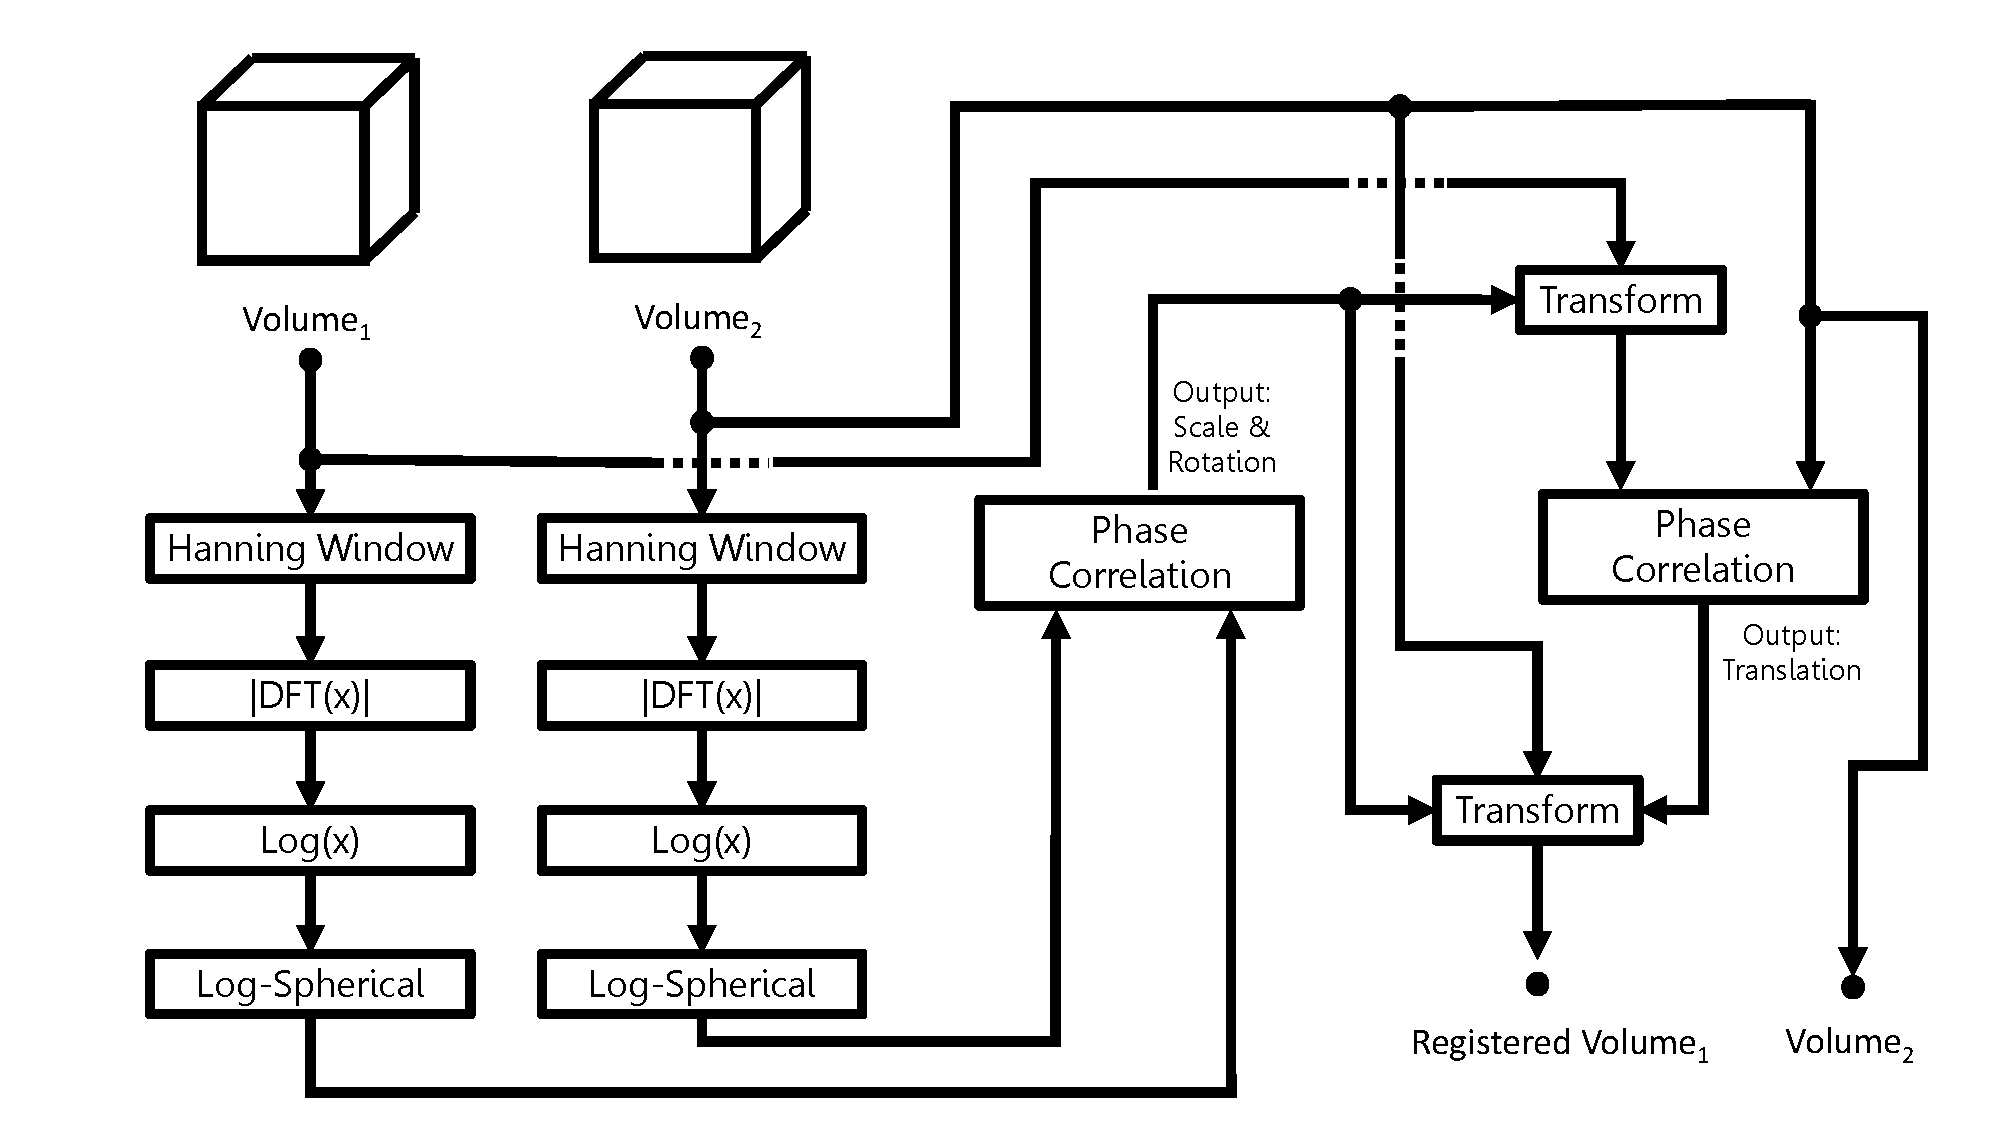
\includegraphics[width=6.0in]{images/ch2/pipeline2}
\caption{System Diagram for Registration Process}
\label{fig:PIPELINE}
\end{figure*}


\subsection{Stereo Camera Based Reconstruction}

\subsection{Monocular Sensor Based 3D Reconstruction}